\section{Basic Usage of the \openshmem Analyzer}
\label{chapter:basic-usage}

In this chapter the user will find:

\begin{itemize}
\item some hints on preparing programs for the \openshmem Analyzer;
\item invoking the \openshmem Analyzer for the first time;
\item naming/graphical conventions;
\item how to visualize the results or manipulate graphs.
\end{itemize}

\subsection{Preparing Your Program for the \openshmem Analyzer}

The first step of preparing a program to be analyzed by the \openshmem
Analyzer is to compile it using the tool with a special set of
flags. The user is responsible for modifying the application's
makefiles, in order to reflect the compiler and flags setting
changes. Since the \openshmem Analyzer is based on OpenUH the
following are the main drivers/compilers:

\vspace{0.1in}

\begin{center}
  \begin{tabular}{|l | l |}
    \hline
    uhcc & C compiler \\
    \hline
    uhCC & C++ compiler (beta evaluation) \\
    \hline
  \end{tabular}
\end{center}

\vspace{0.1in}

In order to prepare your program, you must add the following flags:
-shmem-analyzer -O3 for the compile (-c) and link commands as follows.

\subsubsection*{Compile commands:}

\begin{lstlisting}[language=bash]
  $ uhcc -shmem-analyzer -O3 -c myfile.c
  $ uhcc -shmem-analyzer -O3 -c myfile2.c
\end{lstlisting}

\subsubsection*{Link command:}

\begin{lstlisting}[language=bash]
  $ uhcc -shmem-analyzer -O3 myfile.o myfile2.o -o myprogram 
\end{lstlisting}

Note: To avoid long compilation times, the less aggressive
optimization flag -O2 can be used instead.

In this example, the \openshmem Analyzer will generate a
series of files with extensions: html, gif, dot, map, msg.

This flag will, in future, allow additional information to be passed
into the analyzer, so that analyses specific to a language or library
can be selected.

\subsection{Using the \openshmem Analyzer}

There are~\ref{label:modes} modes of visualizing the results of the \openshmem
Analyzer:
% at the command line or via a web browser.

\begin{enumerate}
\item when you build your program with the \openshmem Analyzer, it
  will display the warnings at the command line;
\item the \openshmem Analyzer is also able to display the warnings in
  a browser together with the program callgraph. \label{label:modes}
\end{enumerate}

\subsubsection{Filename Conventions}

The \openshmem Analyzer creates several files with different extensions. 
The following command:

\begin{lstlisting}[language=bash]
  $ uhcc -shmem-analyzer -O2 myfile.c -o myprogram
\end{lstlisting}

will generate the following files:

\vspace{0.1in}

\begin{center}
  \begin{tabular}{| l | p{10cm} |}
    \hline
    myprogram.html & This is the .html file that can be open with a browser. It contains the callgraph and the warning messages from the tools \\
    \hline
    myprogram.msg & Contains the error messages collected during inter-procedural analysis phase \\
    \hline
    myfile.c.html & This will contain the HTML version of the source code with syntax highlighted and line number target links \\
    \hline
    myfile.c.msg & List of error messages generated during intra-procedural analysis phase \\
    \hline
    myprogram.dot & This file contains the callgraph of the application in the GraphViz format \\
    \hline
    myprogram.gif & This file contains the .gif image version of the callgraph \\
    \hline
  \end{tabular}
\end{center}

\subsection{How the \openshmem Analyzer works}

The \openshmem analyzer relies on intra-procedural and inter-procedural
analysis to detect potential semantic program errors in the
application. The types of warnings reported are displayed during the
different compilation phases of the tool. Figure~\ref{fig:phases} shows
how the different phases generate the different analyses:

\begin{figure}[!ht]
  \begin{center}
    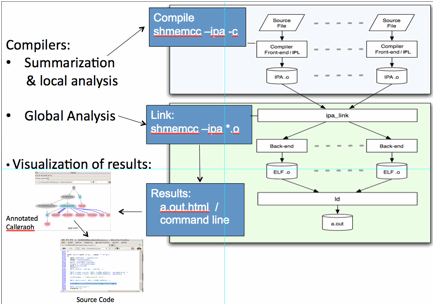
\includegraphics[width=0.5\textwidth]{./image002}
    \caption{Phases generating the different analyses}
    \label{fig:phases}
  \end{center}
\end{figure}

The \openshmem Analyzer generates warning messages at different
compilation stages of the code. The warning messages are then
displayed at the command line or together in the callgraph.  The
\openshmem analyzer does not produce an executable file (in future
releases this feature will be enabled).
